\documentclass[12pt,a4paper]{article}


\usepackage[utf8]{inputenc}
\usepackage[T1]{fontenc}
\usepackage{amsmath}
\usepackage{amsfonts}
\usepackage{amssymb}
\usepackage[francais]{babel}
\usepackage{graphicx}
\usepackage{wrapfig}
\usepackage{hyperref}
\usepackage{cancel}
\usepackage{color}
\usepackage[normalem]{ulem}
\usepackage{soul}
\usepackage[left=2.5cm, right=2.5cm, top=2.5cm, bottom=2.5cm]{geometry}
\usepackage{subfigure}
\usepackage{titletoc}

\author{Baptiste Rouger}
\title{Rapport de stage}
\date{\today}


\begin{document}


	\begin{titlepage}
		
		\begin{center}
			\vfill
			
			{\Huge \textbf{Rapport de stage}}
			
			\vfill
			
			{\LARGE Baptiste \bsc{Rouger}}
			
			~\\L2 BCST
			
			\vfill
			
			{\Huge Analyse de la variation de la hauteur des plantes lors d'une expérience de sélection divergente pour la date de floraison sur le maïs}
			
			\vfill
			
			{\large\today}
			
			\vfill
			\end{center}
			
			\begin{wrapfigure}[5]{l}[12pt]{5cm}
				
\includegraphics[width=5cm]{logo.jpg}
			\end{wrapfigure} ~\\
			UMR de Génétique Quantitative et Evolution - Le Moulon\\
			Ferme du Moulon\\
			91190 Gif-sur-Yvette \\ \\
			
			\begin{figure}[h]
				\centering
				
\includegraphics[width = 4 cm]{inra.jpg}
				
\includegraphics[width = 4 cm]{upsud.jpg}
			\end{figure}
			
			\paragraph*{Directeur de recherche : Olivier \bsc{Martin} \\
			Maître de stage : Christine \bsc{Dillmann}\\
			Enseignant référent : Judith \bsc{Legrand} }
			\vfill
%		\newpage
	\end{titlepage}


	
	\tableofcontents
	\listoffigures
	\newpage
	
		\section*{Glossaire}
		\addcontentsline{toc}{section}{Glossaire}
			\begin{description}
				
				\item [Degré-jour :] unité de mesure utilisée pour calculer l'accumulation de chaleur nécessaire à la durée d'un développement biologique comme la croissance d'une plante.
				
				\item [Dérive génétique :] réduction du nombre de génotypes différents dans une population de taille finie du fait de l'échantillonnage aléatoire des gamètes ou des individus.
				
				\item [Monoïque :] se dit d'une plante dont les fleurs mâles et femelles sont distinctes mais situées sur le même pied.
				
				\item [Mutation :] 
				
				\item [Sélection naturelle :] pression évolutive qui conduit à des changements de la composition génétique d'une population d'une génération à l'autre, en lien avec des différences génétiques des capacités de survie ou de reproduction.
				
			
				
			\end{description}
			
			\newpage
			
		\section{Introduction}
				% faire quelques phrases de présentation ?
				\subsection{Le maïs, une espèce modèle d'intérêt agronomique}
					\subsubsection{Généralités sur le maïs}
						Le maïs (\textit{Zea mays}) est une plante herbacée annuelle appartenant à la famille des \emph{Poacées} (graminées). Par ailleurs, il s'agit d'une plante monoïque.
						
						\paragraph{Cycle de vie du maïs}
						Le cycle de vie du maïs (\bsc{Figure}~\ref{Cycle de vie du maïs en culture}) commence par la phase de dormance du grain, puis sa germination. Vient ensuite le stade végétatif jeune durant lequel la plante développe ses feuilles juvéniles. Il s'achève par la transition florale qui marque le début du stade végétatif adulte. Celui-ci se termine par la floraison débutant le stade reproducteur. Pour finir, lorsque les graines sont mûres, celles-ci peuvent être récoltées.
						\begin{figure}[h]
							\centering
							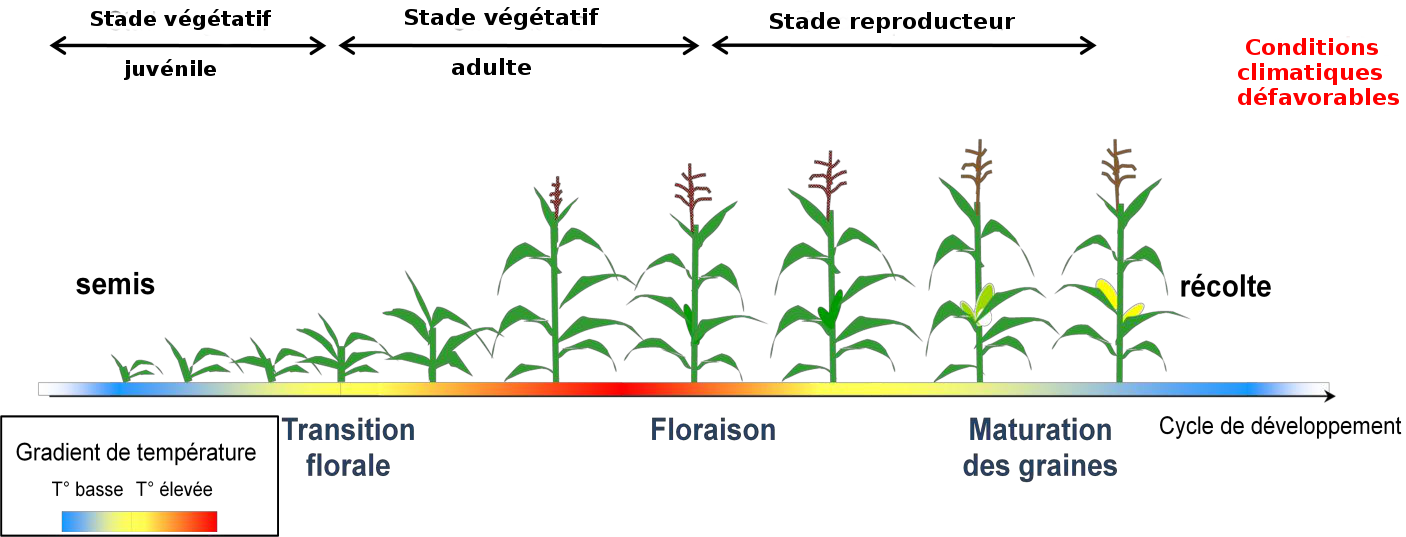
\includegraphics[width=13.7cm]{cycle.png}
							\caption{Cycle de vie du maïs en culture}
							\label{Cycle de vie du maïs en culture}
						\end{figure}
							
					
					\subsubsection{Histoire du maïs}
						Le maïs est une espèce domestiquée depuis environ 9000 ans. Elle est originaire des alentours de Mexico et est issue de la téosinte (\textit{Zea sp}). Elle s'est rapidement propagée à travers le continent américain\cite{tenaillon} en quelques milliers d'années. Cette expansion demanda son adaptation à des climats plus tempérés que son environnement naturel tropical, ce qui fut réalisé en sélectionnant les variétés insensibles à la photopériode, relativement précoces et capables d'effectuer leur cycle de croissance avant l'arrivée des conditions climatiques défavorable (\bsc{Figure}~\ref{Cycle de vie du maïs en culture}). Elle fut découverte et ramenée pour la première fois en Europe par Christophe Colomb lors de sa découverte de l'Amérique. C'est aujourd'hui une des premières céréales cultivées dans le monde.
						
						\paragraph{Domestication du maïs} 
							Lors de sa domestication, le maïs a vu certaines de ses caractéristiques changer pour le voir devenir ce qu'il est aujourd'hui (\bsc{Figure}~\ref{Comparaison entre téosinte et maïs}). On peut par exemple citer l'absence de dissémination de ses graines, l'augmentation de leur poids et de leur nombre, la synchronisation des dates de floraison mâles et femelles ainsi qu'une dominance apicale entraînant une modification de l'architecture de la plante.
							\begin{figure}[h]
								\centering
								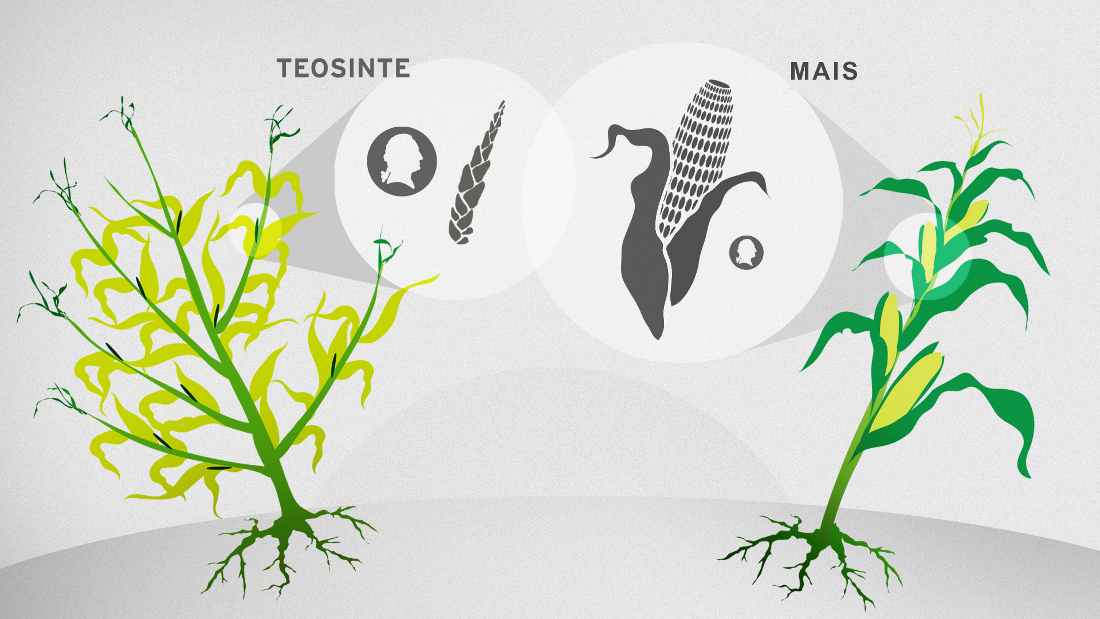
\includegraphics[width=0.5\textwidth]{comparaison.jpg}
								\caption{Comparaison entre téosinte et maïs}
								\label{Comparaison entre téosinte et maïs}
							\end{figure}
	
						
						
			        \subsection{Présentation de l'expérience de sélection divergente}
				
					\subsubsection{Généralités}
						
						%parler des degrés jour pour la mesure des durées pour les plantes.
						\paragraph{Des forces évolutives}
							Les individus d'une population interagissent de façon dynamique avec leur environnement. Ces interactions conduisent à des changements de composition génétique des populations sous l'effet des pressions évolutives. Ainsi, les mutations représentent une pression évolutive puisqu'elles modifient la composition génétique des individus d'une population. De la même façon, on peut citer la dérive génétique et la sélection naturelle, qui amènent à la conservation de certains génotypes.
							
					
					\subsubsection{L'expérience de sélection divergente}
					
						L'expérience de sélection divergente a débuté en 1993. Prenant pour origine deux lignées pures de maïs (F252 et MBS847) à très forte homozygotie, les plants les plus précoces et les plus tardifs pour la date de floraison furent sélectionnés pour le semis chaque année. On obtient ainsi deux populations de maïs pour une même lignée pure, marquants une plus ou moins forte réponse à la sélection selon la variété et la direction de la sélection (\bsc{Figure}~\ref{sélection}). Pour réaliser cette comparaison, la date de floraison est calculée en degré-jour, c'est à dire en somme de température.
						\begin{figure}
							\centering
							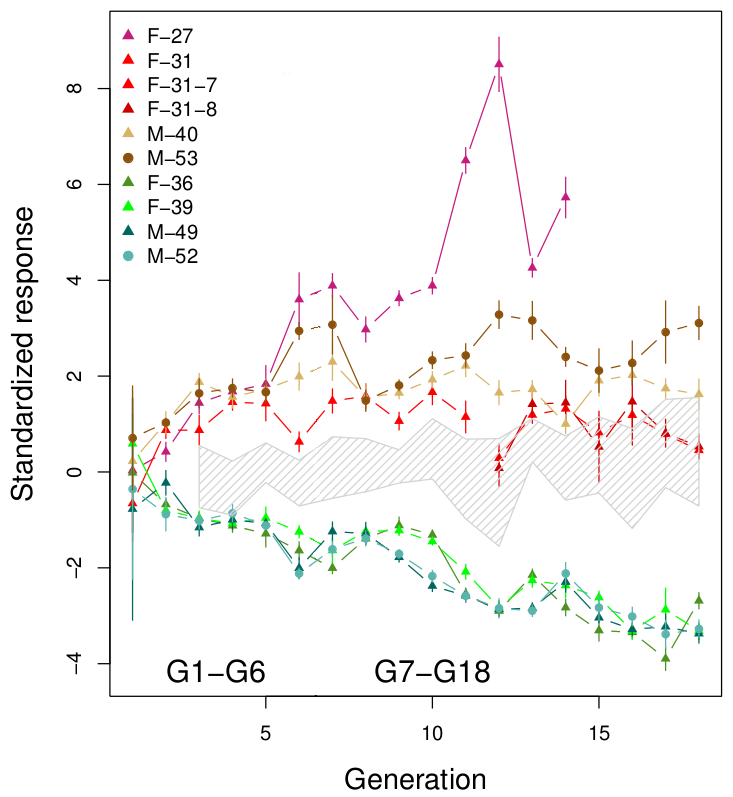
\includegraphics[width =0.5\textwidth]{selection.png}
							\caption{Réponse des deux lignées pures de maïs à la sélection pour la date de floraison}
							\label{sélection}
						\end{figure}
						
						Par ailleurs, la hauteur des plantes fut aussi mesurée, pour observer si, comment, et combien un caractère n'intervenant pas dans la sélection artificielle d'un individu pouvait être modifié par celle-ci.
					
				\subsection{Objectifs du stage}
				
					Une analyse fine des paramètres de hauteur pour chaque population de maïs doit être faite pour déterminer si, comme nous le pensons, la hauteur est corrélée à la date de floraison, et de quelle façon (causale, aléatoire...), et si c'est le cas, dans quelle mesure.
					
			\begin{quotation}
				Après nous êtres intéressés au matériel utilisé lors des vingt années d'expérimentation, nous nous intéresserons au méthodes de traitement des données. Nous analyserons ensuite les résultats et les interpréterons. Enfin, nous conclurons ce sujet.
			\end{quotation}
			
			
			 \section{Matériel et méthodes}
			 		
			 		\subsection{Le matériel végétal}
			 			
			 			L'expérience de sélection divergente (\bsc{Figure}~\ref{selec.div}), débutée en 1993 et toujours en cours, compte 19 générations. Les lignées de départ utilisées sont deux lignées pures à forte homozygotie : les maïs F252 et MBS847 (notée MBS). On obtient pour chaque lignée deux populations, une tardive et une précoce, sélectionnées pour la date de floraison\footnote{Définie lorsque les fleurs mâles et femelles apparaissent} notée en degrés-jours. On replante également chaque année la lignée pure de départ comme témoin.
			 			Par ailleurs, chaque lignée est représentée par plusieurs familles tardives et précoces (\bsc{Figure}~\ref{sélection}) dont le nom est composé d'une lettre suivie de deux ou trois chiffres. Chaque famille est représentée chaque année par un certain nombre de descendants des individus sélectionnés à la génération précédente. Ces individus, appelés \og progéniteurs\fg sont nommés d'une façon qui permet de retracer facilement leur généalogie (\bsc{Figure}~\ref{carte_gen} : chaque point représente un progéniteur sélectionné pour être semé. Les traits entre les points indiquent les relations de parenté entre les progéniteurs. Les derniers progéniteurs sont marqués en noir ainsi que tous leurs ancêtres pour pouvoir retracer leur généalogie.). On a donc plusieurs niveaux d'apparentement : progéniteur, famille, population et lignée.
			 			
			 			A chaque génération, on réalise pour chaque lignée une autofécondation\footnote{Pour réaliser l'autofécondation, on couvre les fleurs des individus de sachets pour recueillir le pollen et protéger les soies. Après vingt-quatre heures, le sachet contenant le pollen est déposé sur la fleur femelle pour réaliser l'autofécondation.} des dix individus les plus précoces et les plus tardifs. Par ailleurs, à chaque génération également, on mesure une dizaine de plantes environ par progéniteur.
			 			
			 			\begin{figure}[h]
			 				
			 				\begin{minipage}[t]{0.45\textwidth}
			 					\centering
			 					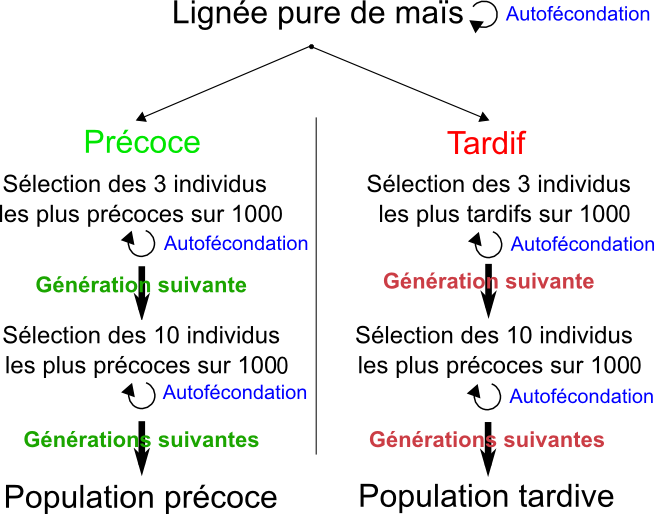
\includegraphics[width=7cm]{selec_div.png} %[width=6.5cm]
			 					\caption{Principe de l'expérience de sélection divergente}
			 					\label{selec.div}
			 				\end{minipage}
			 				\quad
			 				\begin{minipage}[t]{0.45\textwidth}
			 					\centering
			 					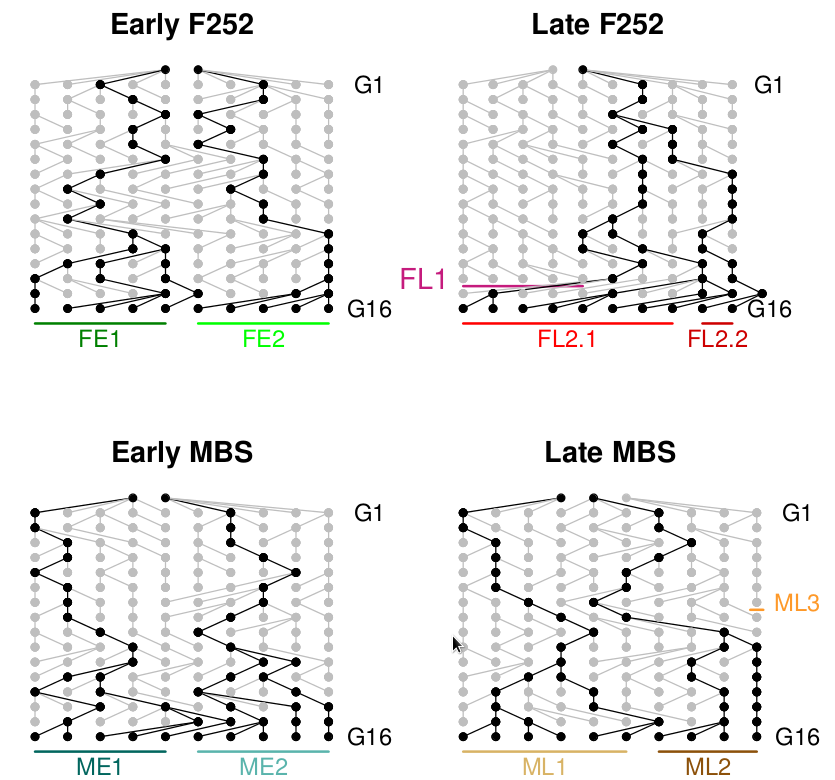
\includegraphics[width=7cm]{carte_gen.png} %[width=6.5cm]
			 					\caption{Généalogie des plantes sélectionnées chez les deux lignées de maïs F252 et MBS pour l'expérience de sélection divergente en 2012}
			 					\label{carte_gen}
			 					
			 				\end{minipage}
			 					
			 
			 
			 				
			 			\end{figure}
			 			
			 		\subsection{Méthodes}
			 			
			 			Pour réaliser les analyses nécessaires à la confirmation de nos hypothèses, il faut commencer par formater toutes les données au même format, c'est à dire que chaque plante mesurée sera référencée avec de nombreuses caractéristiques la concernant : l'année, la génération, la lignée (F252 ou MBS), le parent (c'est-à-dire le \og grand-parent \fg de la plante mesurée), le progéniteur (le parent de la plante), la population à laquelle elle appartient (tardive, précoce ou témoin), la famille qui permet de retracer la généalogie, le bloc, la ligne et le numéro de la plante qui permettent de retrouver la position de la plante dans le champs, et bien évidemment la hauteur de la plante.
			 			
			 			\subsubsection{Mise en forme des données}
			 				
			 				L'ensemble des données, mesurées depuis 1998 et jusqu'en 2014, que l'on doit rassembler se trouve dans des fichiers dont les formats diffèrent du fait de la durée de l'étude. Il faut donc les mettre au même format pour commencer à traiter les données. On choisi le format \textbf{CSV} pour des raisons de commodité. Ces fichiers sont ensuite traités par le script\footnote{Tous les scripts sont réalisés dans le langage interprété par le logiciel d'analyses statistiques \textbf{R}. \textit{cf} \bsc{Annexes}~\ref{scripts}} \textit{\ul{tri.R}}. Celui-ci retourne alors un fichier de données formatées par année. Puis le script \textit{\ul{aggregate.R}} permet de rassembler toutes ces données dans un même fichier au format \textbf{CSV}.
			 			
			 			\subsubsection{Correction des données}
			 				
			 				L'impact de l'année et de l'emplacement dans le champ (appelé \og effet bloc \fg) sur la hauteur des plantes a ensuite été constaté . En effet, il apparaît clair que l'année va jouer un rôle important sur la hauteur de la plante, en fonction de la quantité de précipitations, de la température cumulée, etc. De la même façon, les propriétés du terrain peuvent varier localement, selon par exemple la composition du sol, ce qui va là encore influer sur la hauteur des plantes. Un script\footnote{Il s'agit du script \textit{\ul{DataCorrectv2.R}}} a donc été réalisé pour estimer et corriger les données récoltées.
			 				
			 				Ce script réalise une analyse (effet de l'année et \og effet bloc \fg) de la variance de la hauteur. On utilise ensuite les résultats de cette analyse pour corriger dans un premier temps l'\og effet bloc \fg, et dans un second temps l'effet année. Ceci peut être fait grâce aux plantes témoins dont la hauteur moyenne ne devrait pas varier d'une année sur l'autre.Cela permet également de vérifier que la correction des données est efficace.
			 				
			 		\subsection{Résultats}
			 			
			 			\subsubsection{Réponse de la hauteur des plantes à la sélection pour la date de floraison}
			 				
			 				Les deux figures suivantes (\bsc{Figures}~\ref{hauteursf252} et ~\ref{hauteursmbs}) représentent par des boxplots les variations de la hauteur des individus mesurés pour chaque population en fonction du temps. Elles présentent également la pente de la variation des hauteurs au cours du temps (on peut trouver le coefficient directeur de cette droite en haut de chaque graphe).\\
			 				Si l'on observe les témoins, on remarque que le coefficient de leur droite de régression est de zéro (avec une certitude de rejet de H$_{1}$(variation de hauteur en fonction du temps) de 100\%). On peut ainsi dire que les données on bien été corrigées puisque les hauteurs des témoins sont stables et invariées au cours du temps.\\
			 				
			 				On observe également ( \bsc{Figure}~\ref{hauteursf252} et \bsc{Figure}~\ref{hauteursmbs} ) des tendances à la hausse pour les populations tardives (0.53 cm/an et 0.21 cm/an respectivement pour F252 et MBS)  et une tendance à la baisse pour la population précoce de MBS (-0.64cm/an). La population précoce de F252 semble cependant augmenter de taille, bien que très faiblement (0.03cm/an).\\		 				
			 				Ainsi, les variations des hauteurs des plantes au cours du temps sont très faibles d'année en année pour l'ensemble des données observées. Or on constate, particulièrement pour les lignées tardives, que la hauteur des plantes est déjà différente de la hauteur du témoin pour la première année d'observation des hauteurs. Cela semble indiquer qu'une réponse très rapide à la sélection a eu lieu dans les premières années, puis que cette réponse a très rapidement diminué voire cessé.
			 				
			 				
			 				\begin{figure}[h]
			 					\begin{minipage}[t]{0.32\textwidth}
			 						\subfigure[Population précoce]{
			 							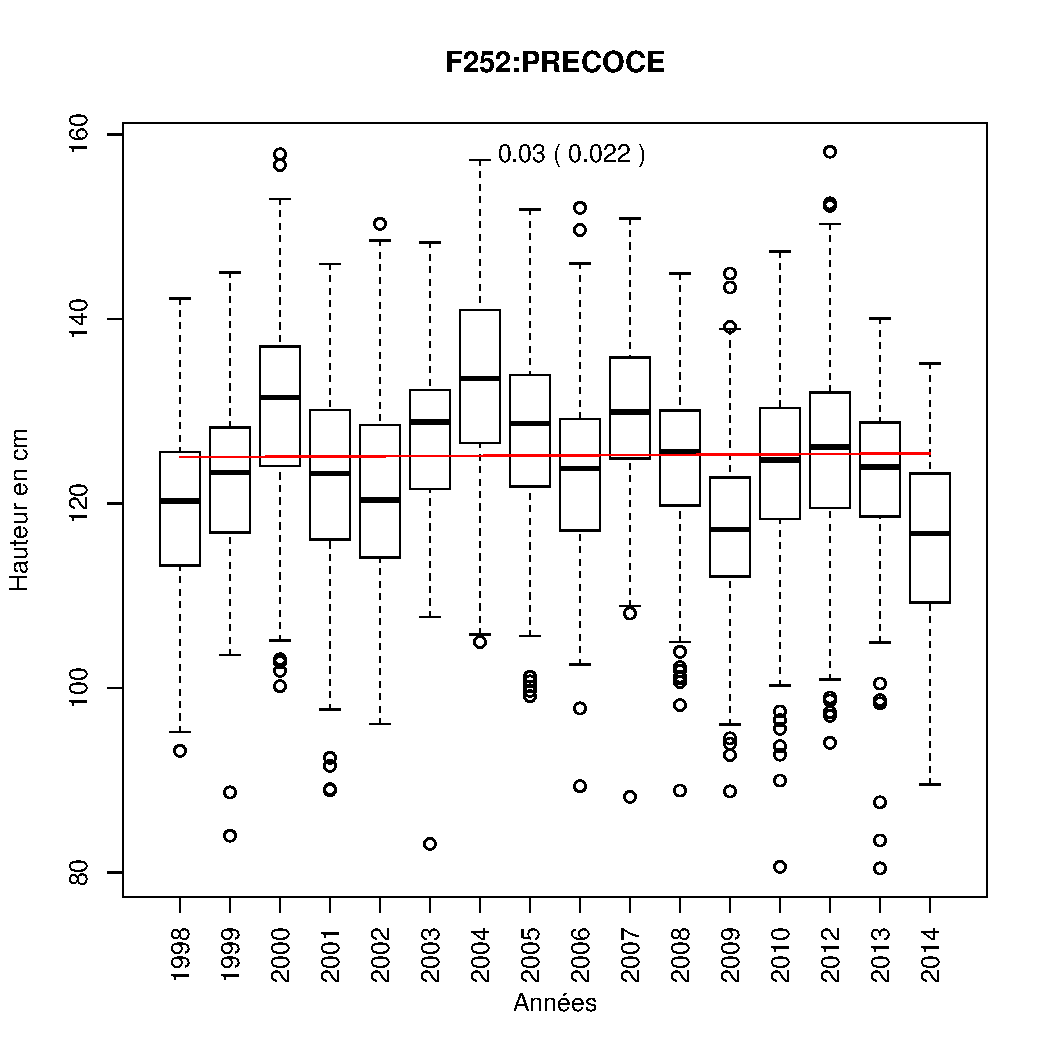
\includegraphics[width=4.5cm]{plot_haut_pop_F252_PRECOCE.pdf}
			 						}
			 					\end{minipage}
			 					\begin{minipage}[t]{0.32\textwidth}
			 						\subfigure[Population témoin]{
			 							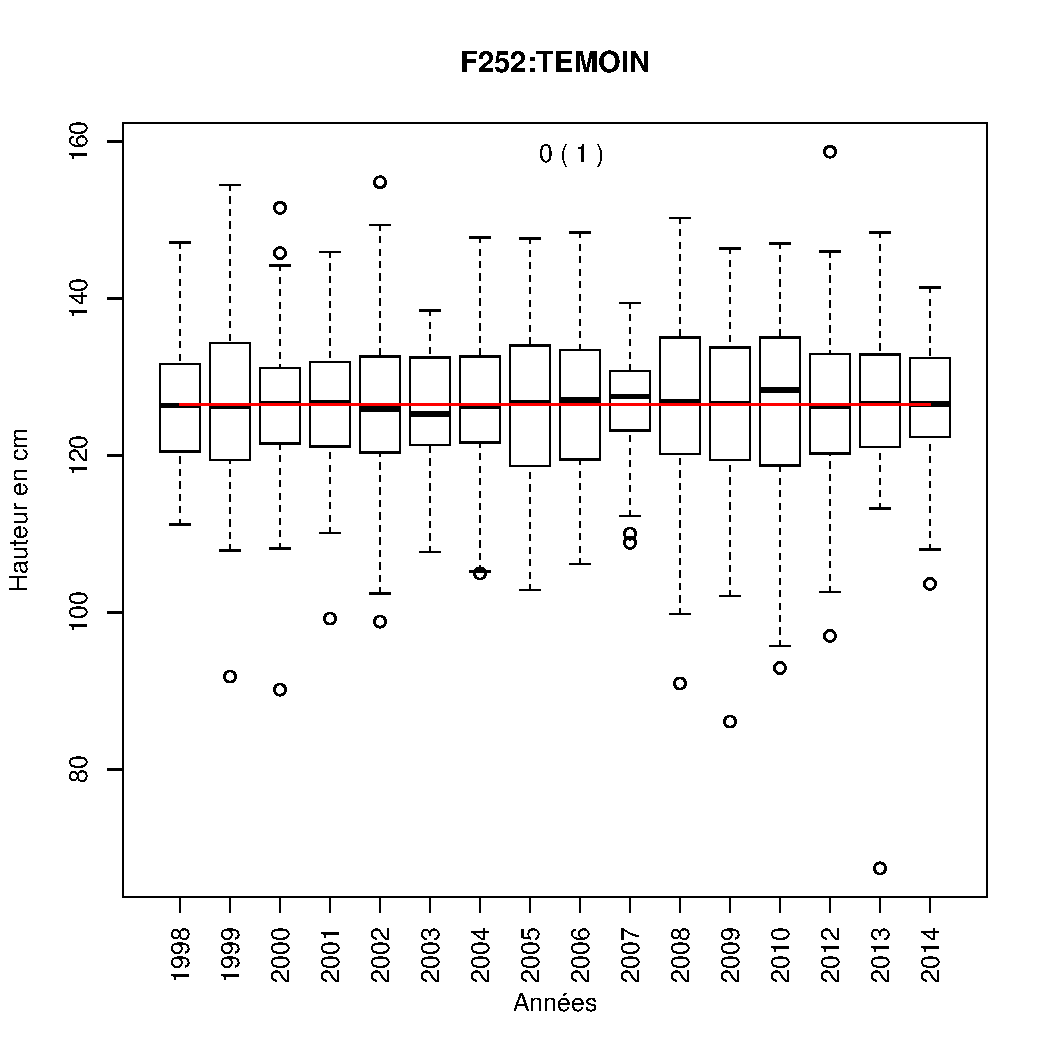
\includegraphics[width=4.5cm]{plot_haut_pop_F252_TEMOIN.pdf}
			 						}
			 					\end{minipage}
			 					\begin{minipage}[t]{0.32\textwidth}
			 						\subfigure[Population tardif]{
			 							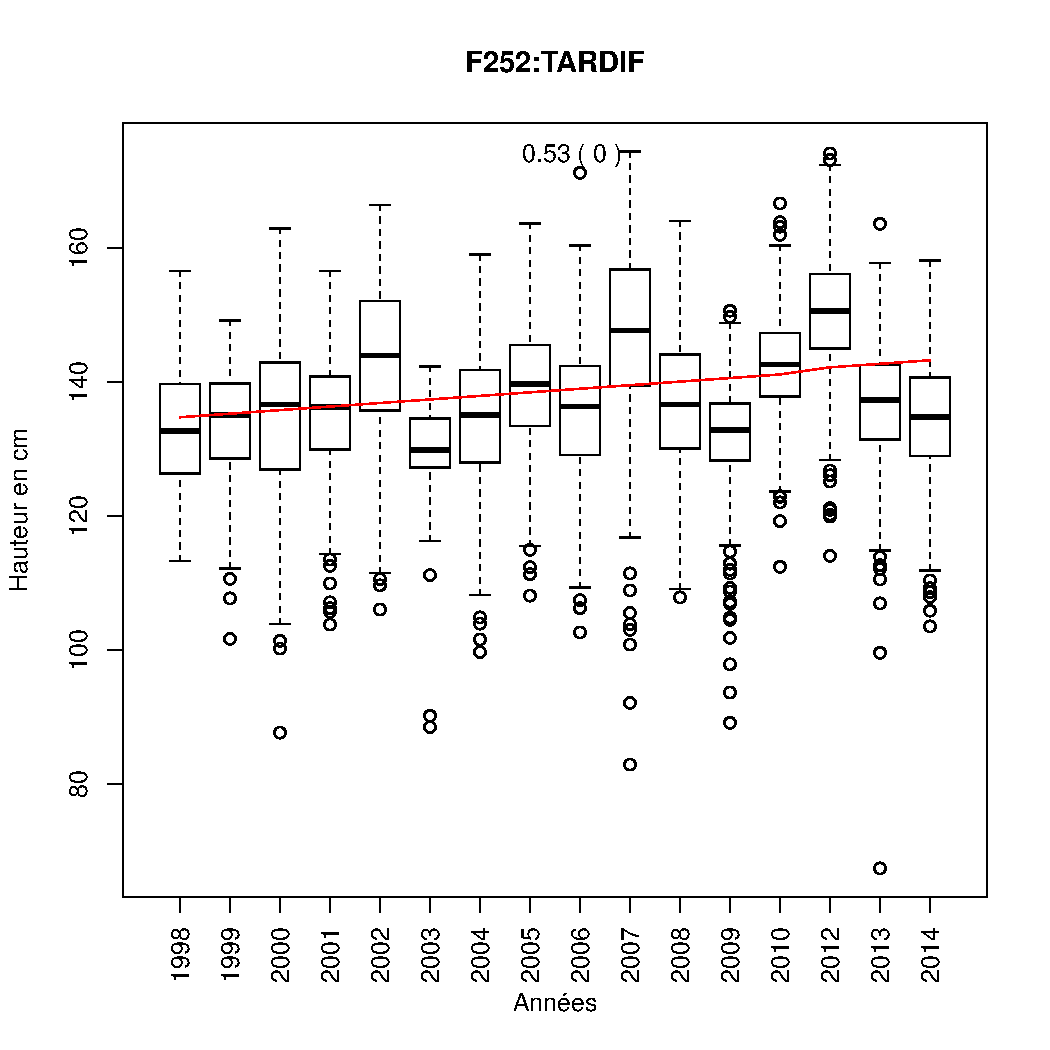
\includegraphics[width=4.5cm]{plot_haut_pop_F252_TARDIF.pdf}
			 						}
			 					\end{minipage}
			 					\caption{Représentation des hauteurs des plantes de la lignée F252 \label{hauteursf252}}
			 				\end{figure}
			 				\begin{figure}[h]
			 					\begin{minipage}[t]{0.32\textwidth}
			 						\subfigure[Population précoce]{
			 							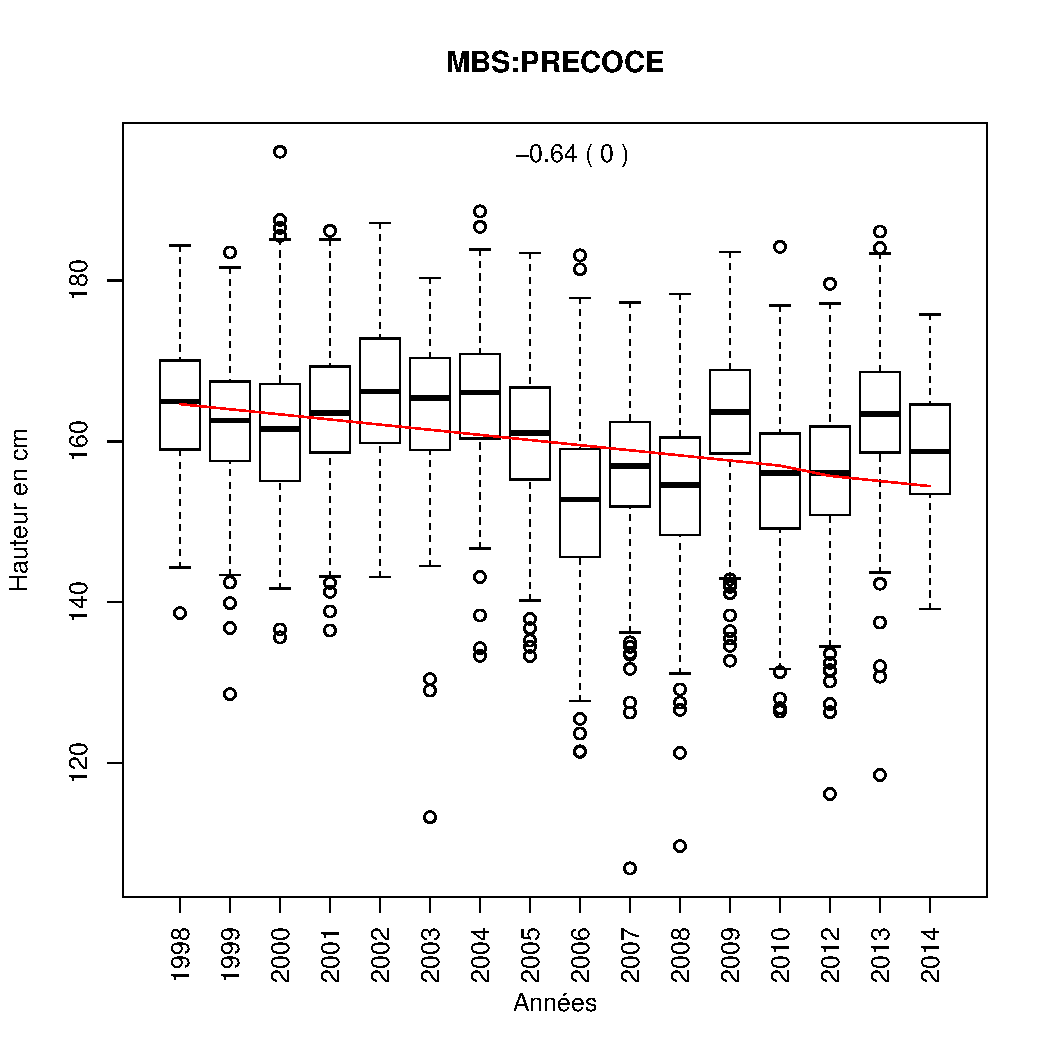
\includegraphics[width=4.5cm]{plot_haut_pop_MBS_PRECOCE.pdf}
			 						}
			 					\end{minipage}
			 					\begin{minipage}[t]{0.32\textwidth}
			 						\subfigure[Population témoin]{
			 							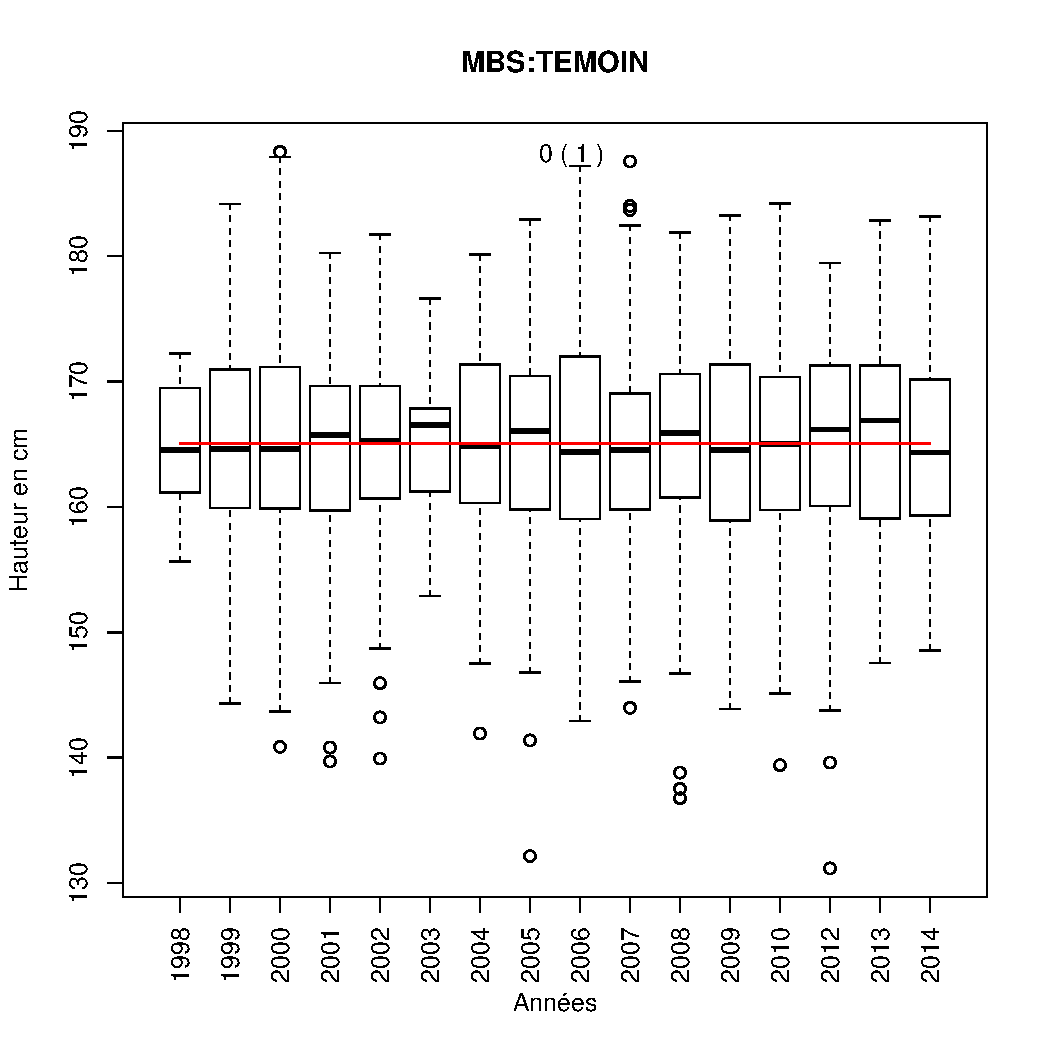
\includegraphics[width=4.5cm]{plot_haut_pop_MBS_TEMOIN.pdf}
			 						}
			 					\end{minipage}
			 					\begin{minipage}[t]{0.32\textwidth}
			 						\subfigure[Population tardif]{
			 							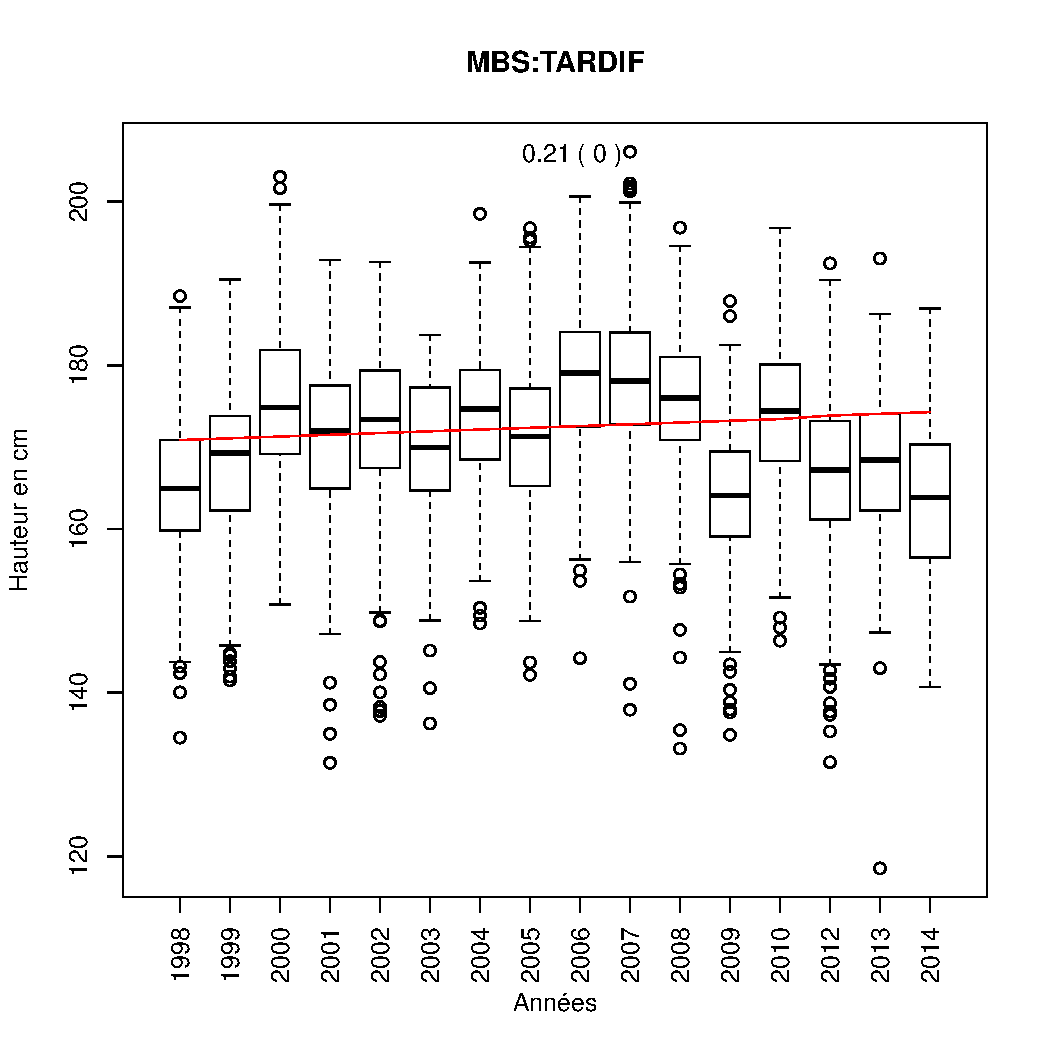
\includegraphics[width=4.5cm]{plot_haut_pop_MBS_TARDIF.pdf}
			 						}
			 					\end{minipage}
			 					\caption{Représentation des hauteurs des plantes de la lignée MBS \label{hauteursmbs}}
			 				\end{figure}
			 
			 			\subsubsection{Corrélation entre hauteur et date de floraison}
			 				
			 				\paragraph{Corrélation par famille et par année}
			 				Il a également été testée si il y avait bien une corrélation entre la hauteur des plantes et la date de floraison (\bsc{Figure}~\ref{correlation}). Pour cela, on a représenté pour chaque famille et chaque année la hauteur moyenne des plantes en fonction de leur date moyenne de floraison.\\
			 				On observe ainsi une répartition globale des points autour d'une droite. On peut également observer une scission entre les populations précoces et tardives des lignées (respectivement représentées dans des couleurs froides et des couleurs chaudes en \bsc{Figure}~\ref{correlation}). Par ailleurs, il semble qu'il n'y ait pas forcément de corrélation intra-famille.\\
			 				Cela confirme donc le fait que la hauteur et la date de floraison sont corrélées pour les lignées.
			 				
			 				\begin{figure}[!h]
			 						\subfigure{
			 							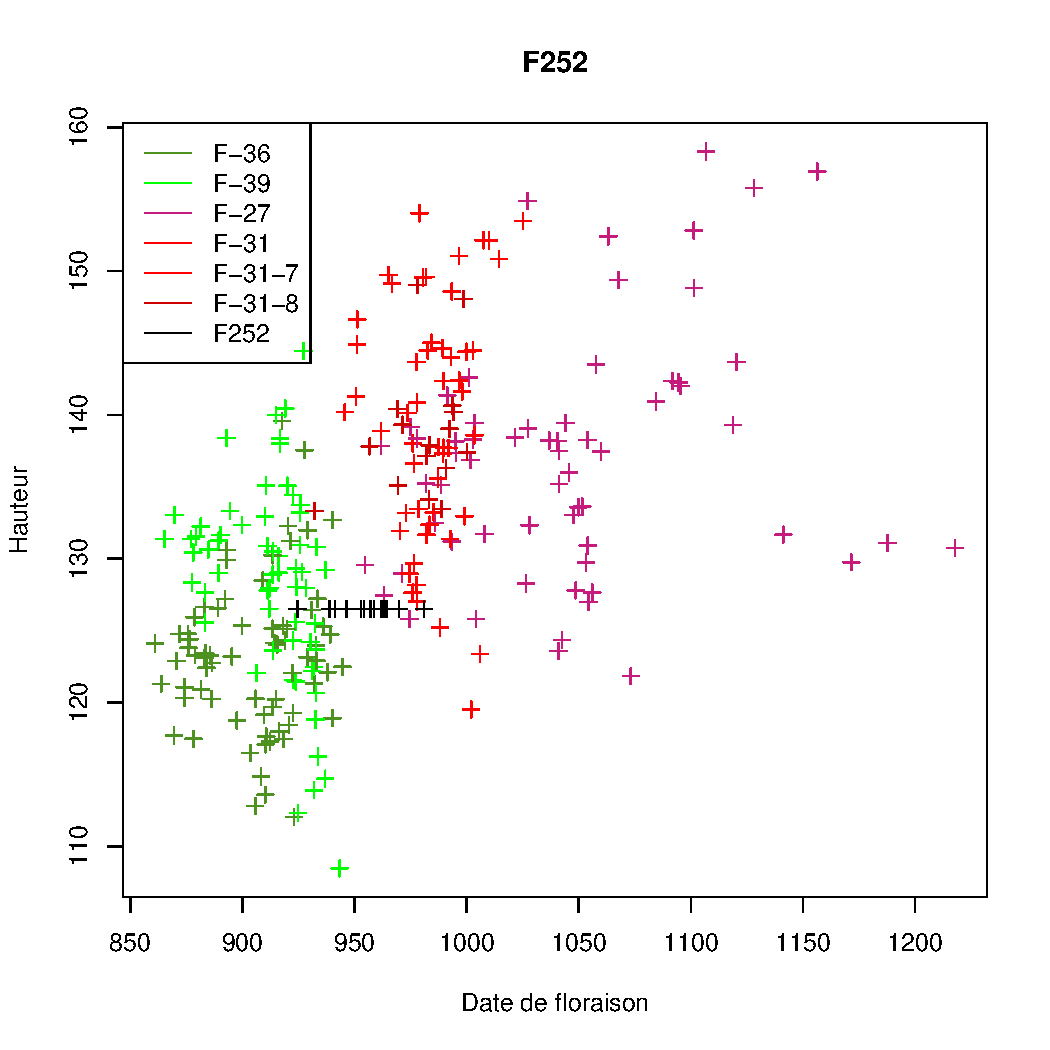
\includegraphics[width=0.45\textwidth]{plot_haut-flo_F252.pdf}
			 						}
			 						\subfigure{
			 							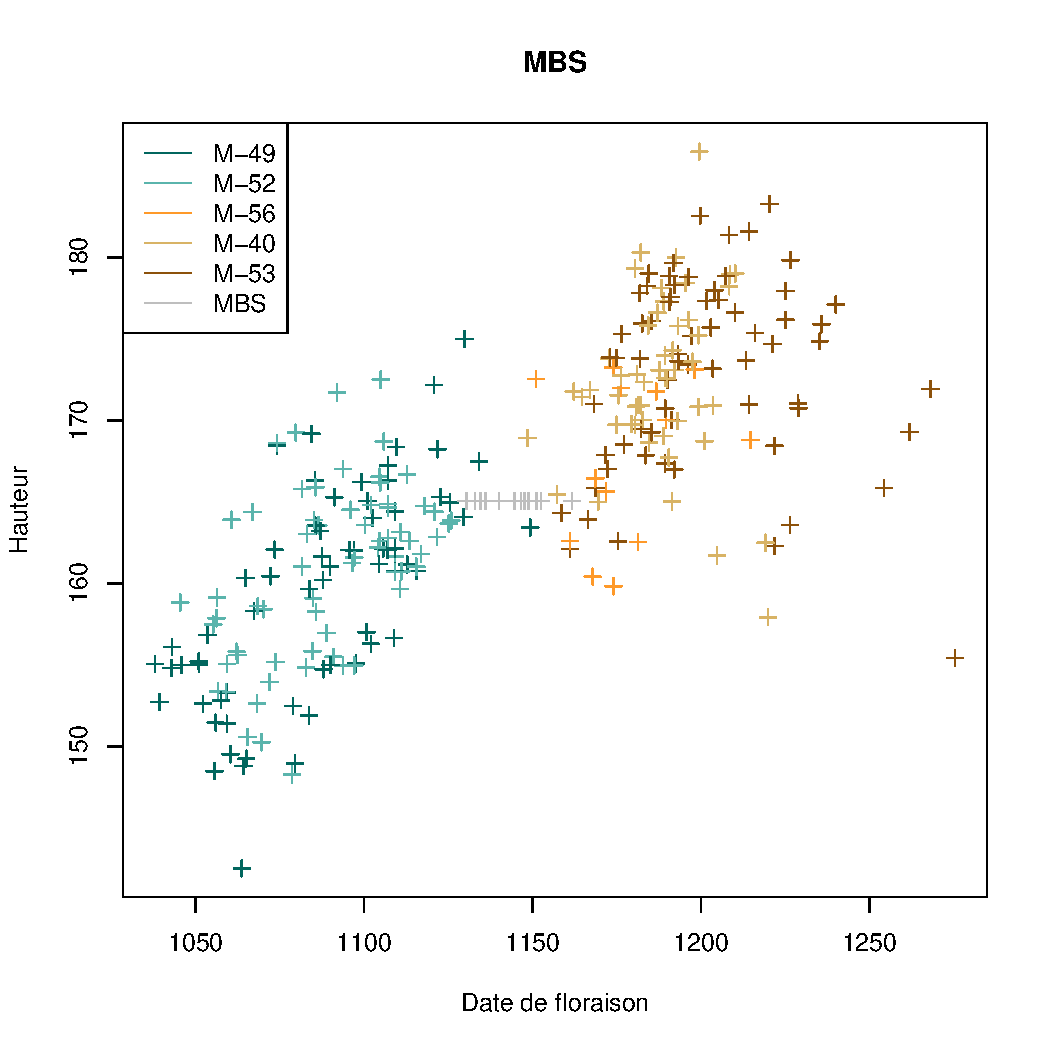
\includegraphics[width=0.45\textwidth]{plot_haut-flo_MBS.pdf}
			 						}
			 					\caption{Représentation de la relation entre hauteur et date de floraison \label{correlation}}
			 					Chaque point d'une couleur représente la moyenne de la hauteur des progéniteurs d'une famille pour une année (couleurs dans la figure) en fonction de la date moyenne de floraison de ces mêmes plantes. A gauche, la lignée F252 et à droite la lignée MBS.
			 				\end{figure}
			 				
			 				\paragraph{Corrélation intra-famille}
			 					
								En \bsc{Figure}~\ref{correl.fam}, on a représenté pour deux familles précoces (F-39 et M-49) l'évolution de la relation entre hauteur et date de floraison en indiquant l'année par des nombres. Ainsi, on peut suivre l'évolution de la corrélation. On observe ainsi que les points ne semblent pas évoluer dans le même sens pour la hauteur : on voit F252 augmenter puis se stabiliser, tandis que MBS voit sa hauteur descendre de façon semble-t-il constante. Il semble donc qu'il n'y ait pas de réelle corrélation entre la hauteur et la date floraison.
			 				
			 				
			 				\begin{figure}[!h]
			 					\subfigure[Famille F-39]{
			 						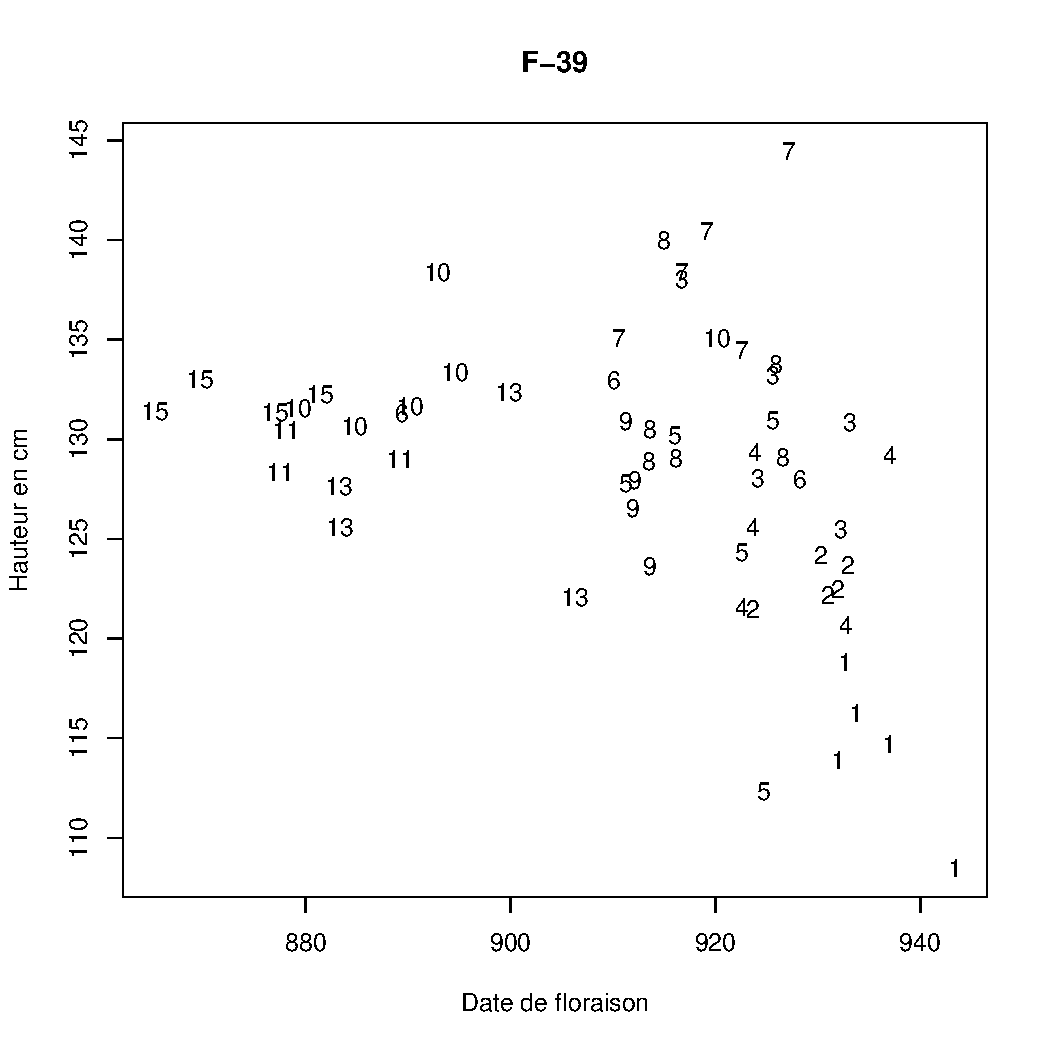
\includegraphics[width=0.45\textwidth]{plot_haut-flo_f39.pdf}
			 					}
			 					\subfigure[Famille M-49]{
			 						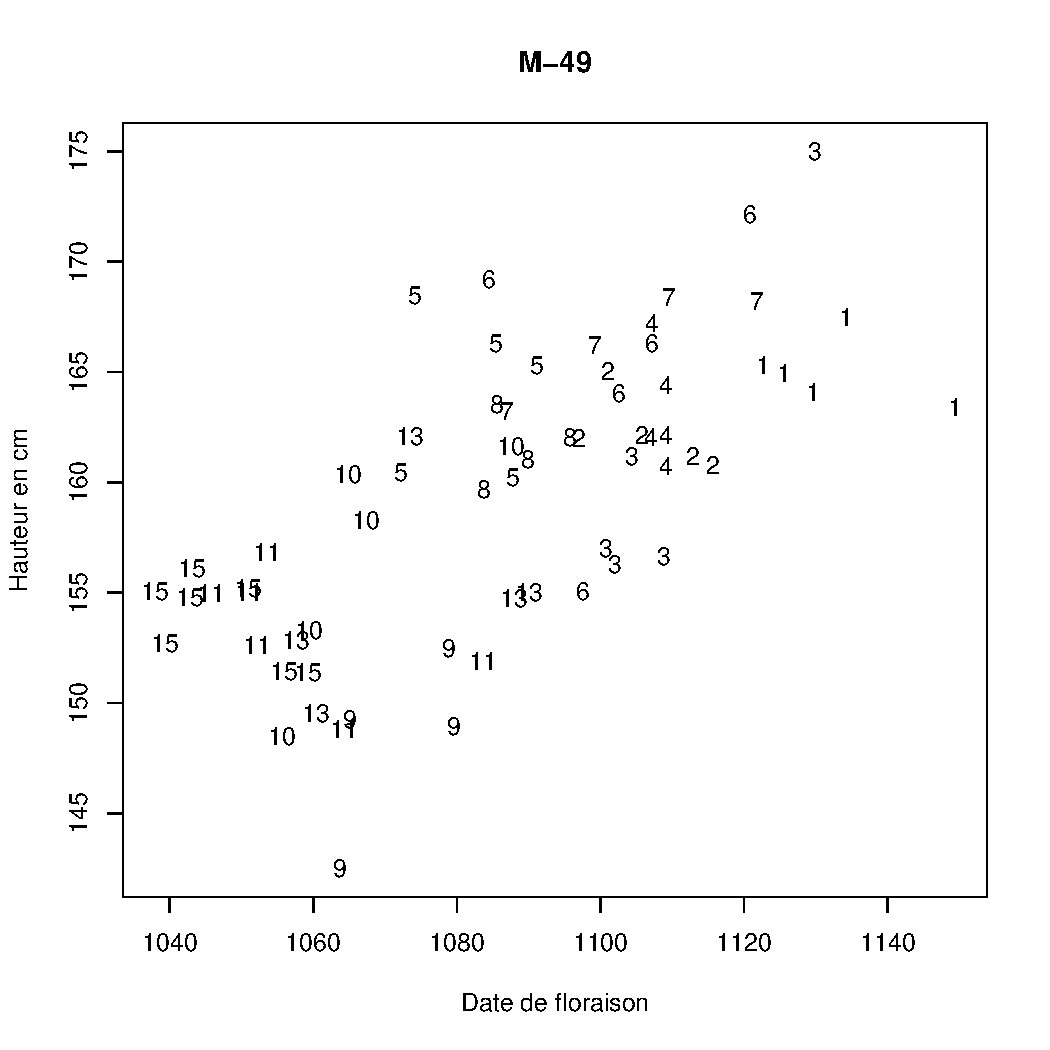
\includegraphics[width=0.45\textwidth]{plot_haut-flo_m49.pdf}
			 					}
			 					\caption{Représentation séparée de la corrélation entre hauteur et date de floraison pour deux familles \label{correl.fam}}
			 					Chaque nombre représente par sa position la moyenne de la hauteur des progéniteurs de la famille (F-39 à gauche et M-49 à droite) en fonction de la date de floraison. Les nombres indiquent l'année (1998 étant l'année 1), on peut donc suivre l'écolution de la corrélation au cours du temps.
			 				\end{figure}
			 				
			 			\paragraph{Corrélation par plante pour 2013 et 2014}
			 				
			 				Les \bsc{Figures}~\ref{correlf252} et ~\ref{correlmbs} présentent les coefficients de corrélation de chaque famille pour les années 2013 et 2014 pour les deux lignées. Il s'agit de données mesurée plante par plante et non corrigées.
			 				Si l'on regarde tout d'abord au niveau global (c'est à dire sur l'ensemble de la lignée de l'année), on remarque que la corrélation est toujours significative à 95\% et positive. A l'échelle des populations (précoce, témoin et tardif), on peut observer des inconstances dans les corrélations. Ainsi, pour F252, on peut voir que les tardifs ont une corrélation non significative pour les deux années, alors que les populations précoce et témoin ont un coefficient de corrélation tantôt significatif, tantôt non significatif. Pour MBS, on remarque que la population précoce reste corrélée de façon significative et que la population témoin a un coefficient de corrélation qui reste non significatif. On voit également, cependant, que la population témoin est tantôt significative, tantôt non significative.\\
			 				Quant aux familles, elles ont un coefficient de corrélation pour la plupart non significatif. On observe cependant des années où les familles sont corrélées de façon significative, sans lien avec les autres années.\\
			 				De même, on peut observer que, pour certaines familles et populations, les coefficients de corrélation sont tantôt positifs, tantôt négatifs.\\
			 				
			 				\begin{figure} [!h]
			 					\subfigure[Année 2013]{
			 						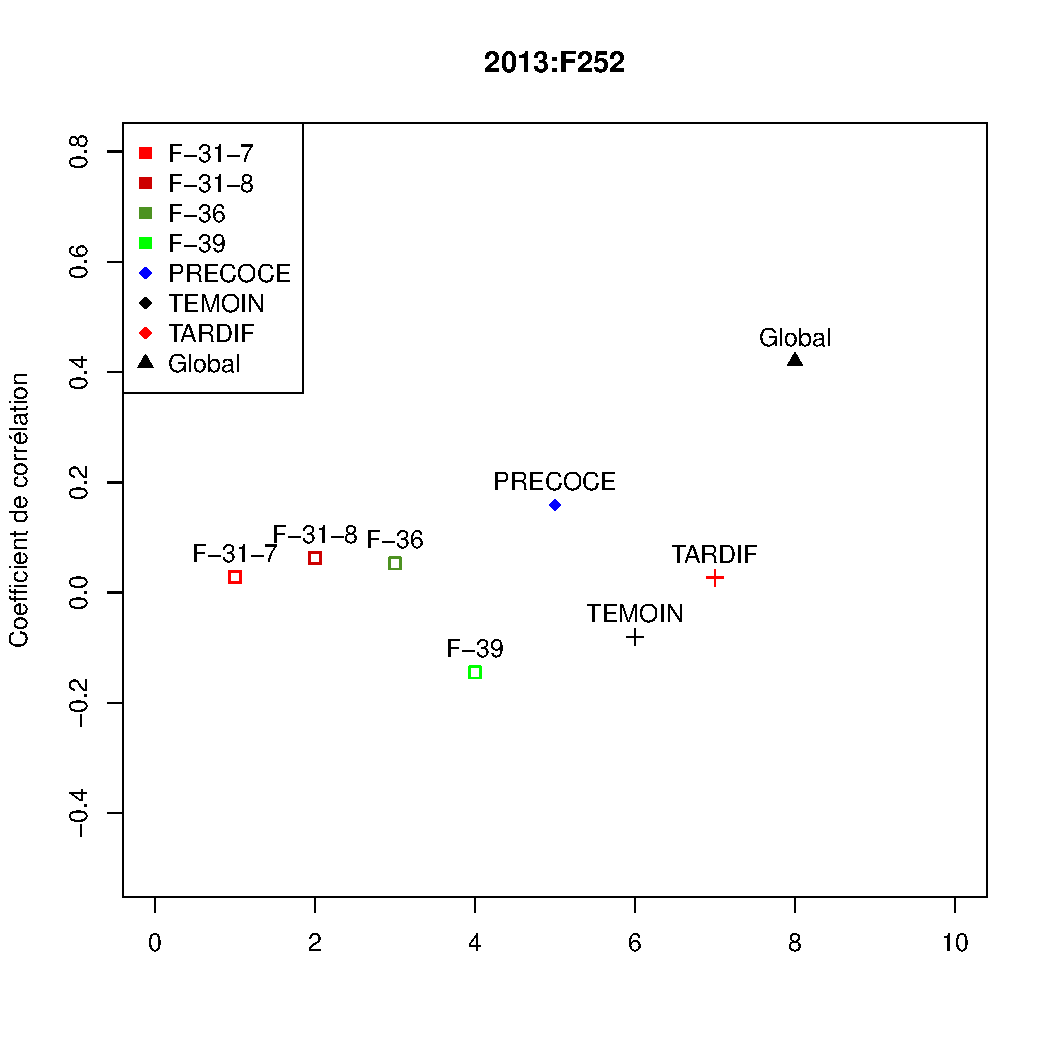
\includegraphics[width=0.45\textwidth]{F2522013.pdf}
			 					}
			 					\subfigure[Année 2014]{
			 						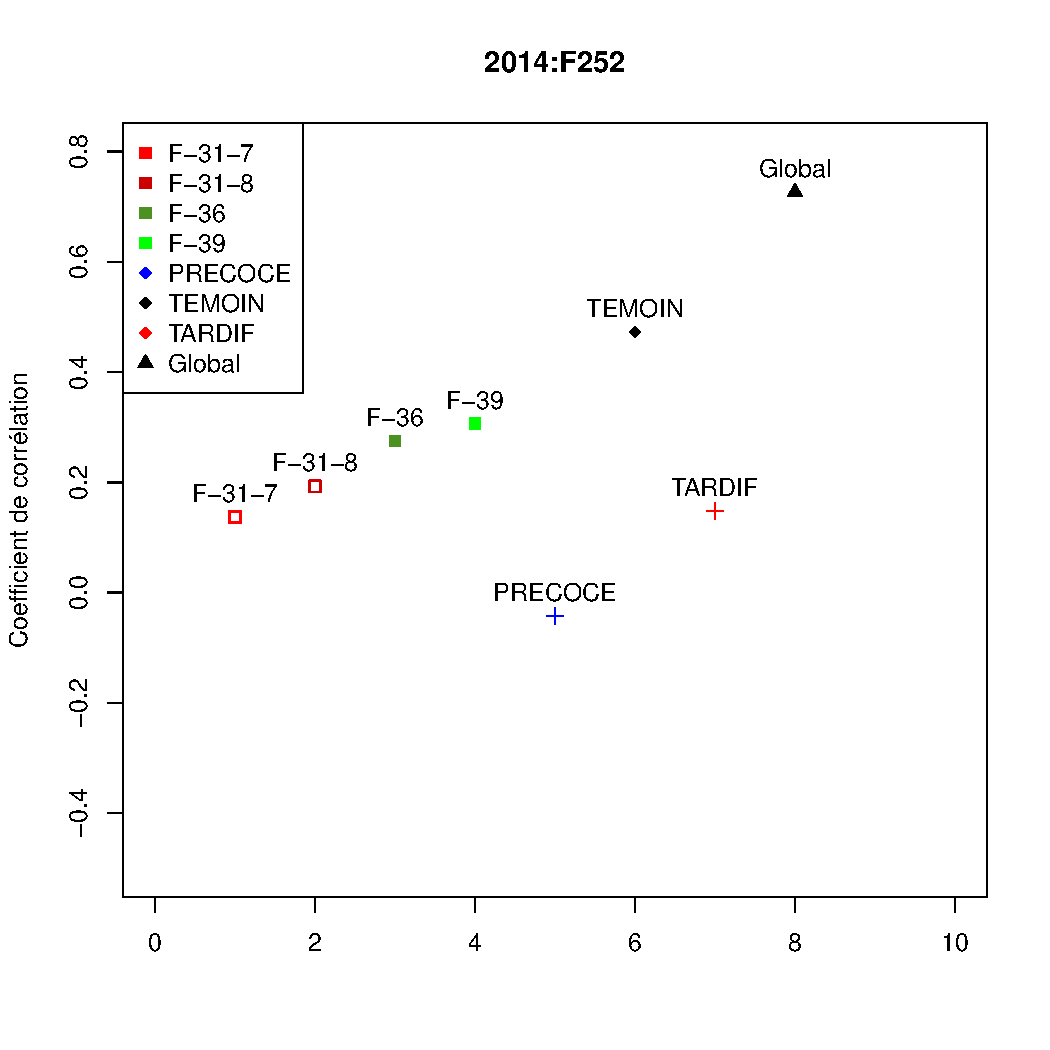
\includegraphics[width=0.45\textwidth]{F2522014.pdf}
			 					}
			 					\caption{Répresentation des coefficients de corrélation entre hauteur et date de floraison par plante en 2013 et 2014 pour F252 \label{correlf252}}
			 					Le coefficient de corrélation de chaque famille, calculé en associant la hauteur et la date de floraison de chaque plante, est représenté en figuré plein si la corrélation est significative à 95\% et en figuré creux si la corrélation n'est pas significative pour le même seuil.
			 				\end{figure}
			 				\begin{figure} [!h]
			 					\subfigure[Année 2013]{
			 						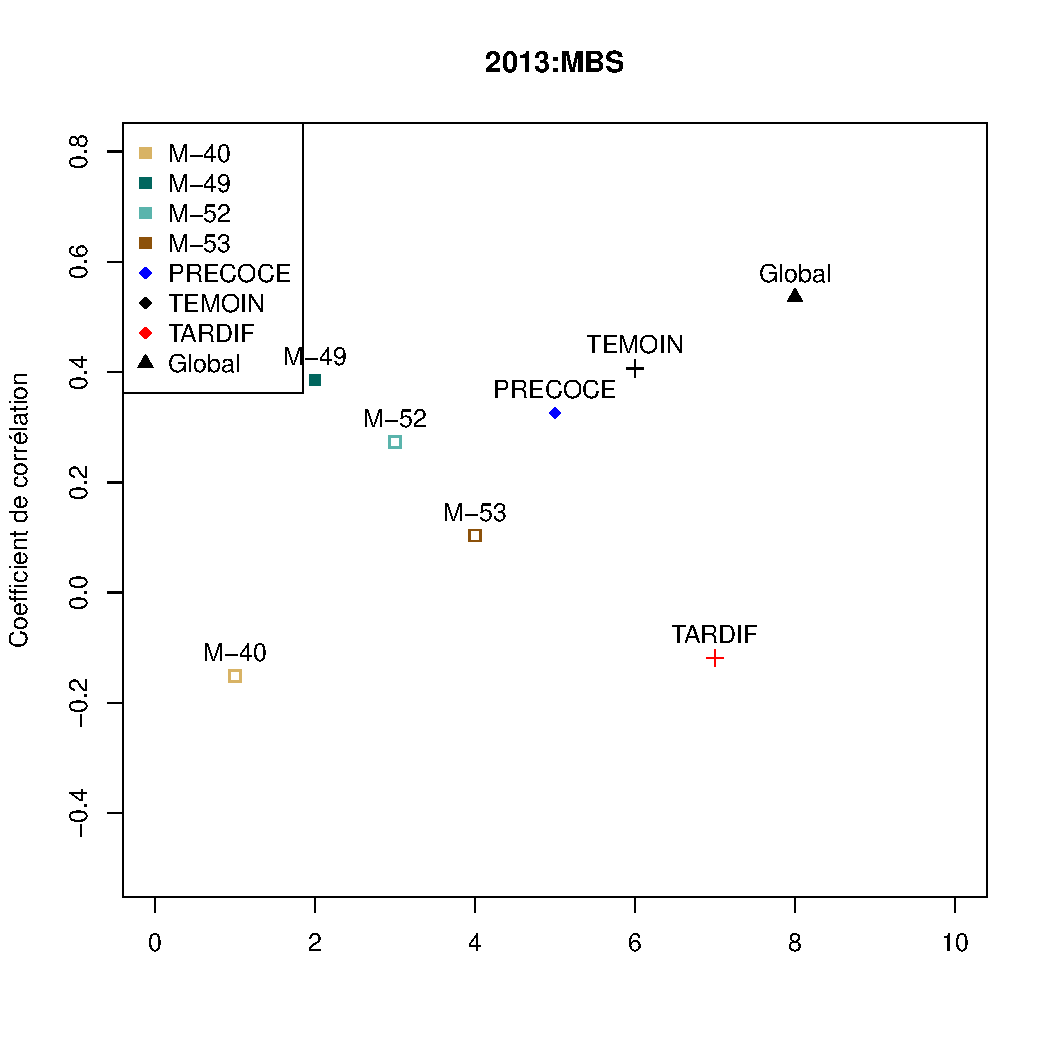
\includegraphics[width=0.45\textwidth]{MBS2013.pdf}
			 					}
			 					\subfigure[Année 2014]{
			 						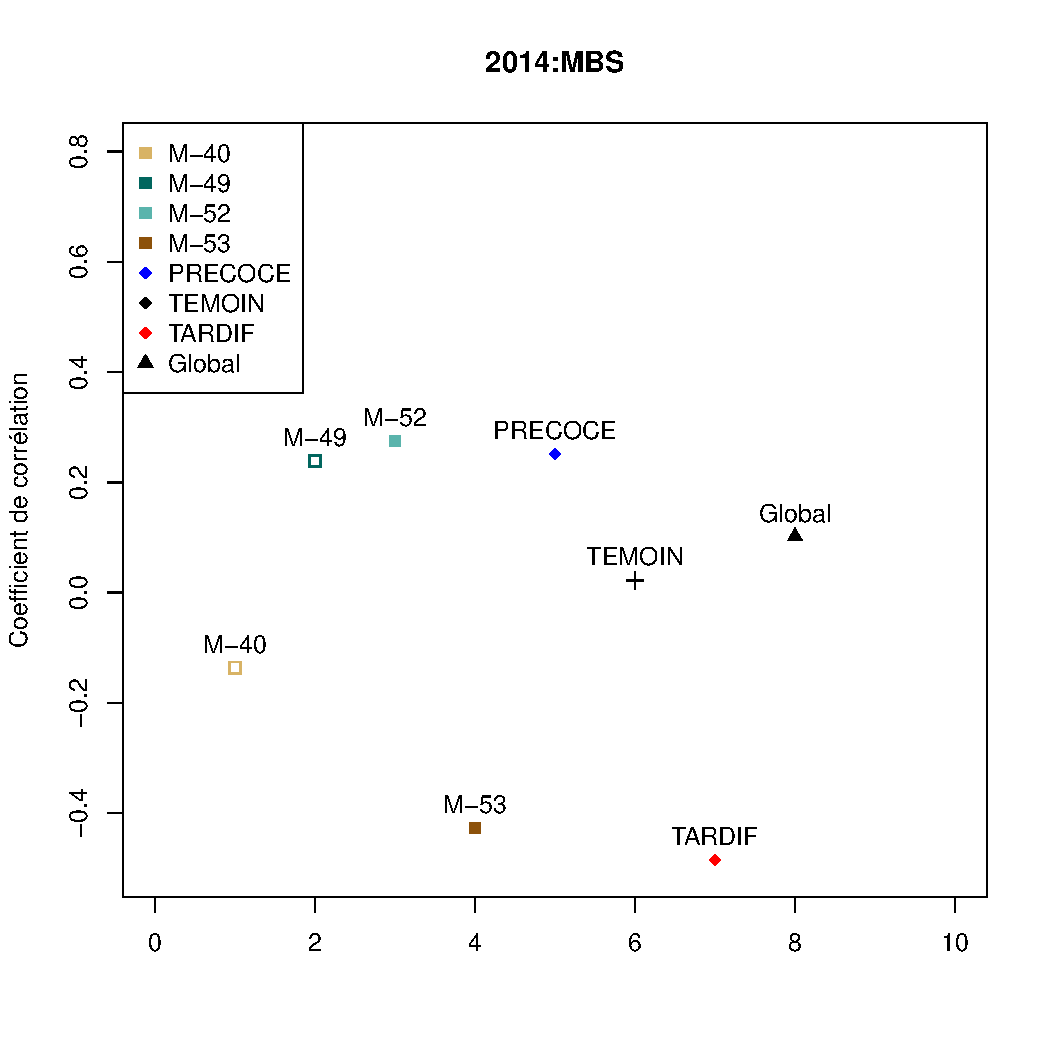
\includegraphics[width=0.45\textwidth]{MBS2014.pdf}
			 					}
			 					\caption{Répresentation des coefficients de corrélation entre hauteur et date de floraison par plante en 2013 et 2014 pour MBS \label{correlmbs}}
			 					Le coefficient de corrélation de chaque famille, calculé en associant la hauteur et la date de floraison de chaque plante, est représenté en figuré plein si la corrélation est significative à 95\% et en figuré creux si la corrélation n'est pas significative pour le même seuil.
			 				\end{figure}
			 				
			 				On peut donc dire qu'il n'y a pas de corrélation intra-famille ou populationnelle entre la hauteur et la date de floraison. Cependant, sur l'ensemble des plantes, on peut confirmer l'existence d'une corrélation entre la hauteur et la date de floraison.
			 	\section{Discussion}
			 		
			 		On a donc pu conclure à une corrélation entre la hauteur et la date de floraison sur l'ensemble des plantes d'une lignée, et ce de façon certaine puisque celle-ci apparaît toujours de façon positive et significative, mais que cette corrélation n'existait pas avec certitude à l'intérieur des populations et des familles. Si le biais échantillonnage parait improbable (les échantillons vont de quelques centaines d'individus à des milliers d'individus mesurés), un biais a pu être introduit lors de la correction des données, ce qui induirait une erreur dans les tests et les représentations. De la même façon, lors de l'analyse de la corrélation par plante pour 2013 et 2014,  les données n'ont pas été corrigées, et un biais a pu être introduit par \og effet bloc\fg  ou \og effet année\fg. Il pourrait donc être important de corriger ces données.\\
			 		
			 		Nous avons vu qu'une corrélation entre hauteur et date de floraison existait pour les lignées. Il serait intéressant de voir si le nombre de feuille et/ou la longueur des entre-n\oe{}uds a été modifiée par l'expérience de sélection divergente pour la date de floraison.
			 		
			 	\section{Conclusion}
			 		
			 		Nous avons donc montré qu'une corrélation, comme nous le pensions, existait entre la hauteur et la date de floraison, mais que celle-co n'existait qu'au niveau des lignées, et pas au niveau des familles. Nous n'avons pu conclure à la source de cette corrélation.
	
	\newpage
			
	\bibliographystyle{plain}
	\bibliography{rapport}
	
	\newpage
	\appendix
		
		\section{Codes sources}
		\label{scripts}
		Les codes sources utilisés pendant ce stage sont disponibles sur Github à l'adresse suivante : \url{https://github.com/rougerbaptiste/stageL2}.\\~\\
		Voici la fonction de chacun de ces codes :
		\begin{description}
			\item [aggregate.R :] Ce script a pour fonction de rassembler les données contenues dans les fichiers de hauteurs de chaque année pour les rassembler dans un unique fichier.
			\item [Datacorrectv2.R :] Ce script corrige les données des années et affiche un graphe (\textit{Référence}) résumant les données.
			\item [RprFam.R :] Ce script a pour fonction de représenter les données de hauteurs obtenues pour chaque famille (hauteur absolue et hauteur relative au témoin) et de créer un fichier .pdf contenant les deux graphes.
			\item [RprPop.R :] Ce script a pour fonction de représenter les données de hauteurs obtenues pour chaque population (hauteur absolue et hauteur relative au témoin) et de créer un fichier .pdf contenant les deux graphes.
			\item [tri.R :] Ce script a pour fonction de récupérer toutes les données brutes de hauteurs, de les mettre sous une forme standard et de créer un fichier contenant les données de hauteur par année.
			
		\end{description}

\end{document}
